\documentclass[a4paper,11pt]{article}
%\documentclass[a4paper,11pt,twocolumn]{article}%twocolumn layout; not sure if this works correctly. Feel free to experiment.
\usepackage[pdftex]{color,graphicx}
\usepackage[T1]{fontenc}
\usepackage{pxfonts}
\usepackage{subfigure}
\usepackage{xcolor}

%color links to figs, etc.
\usepackage[pdftex,colorlinks]{hyperref}
\hypersetup{colorlinks,%
            citecolor=black,%
            filecolor=black,%
            linkcolor=black,%
            urlcolor=black,%
            breaklinks=true,%
            pdftex}
            
%easily manipulate margins
\usepackage{geometry}
\makeatletter
\if@twocolumn%
    \geometry{twoside,
        paperwidth=210mm,
        paperheight=297mm,
        textheight=682pt,
        textwidth=516pt,
        centering,
        headheight=50pt,
        headsep=12pt,
        footskip=18pt,
        footnotesep=24pt plus 2pt minus 12pt,
        columnsep=14pt} 
\else%if using twocolumns, I still need to modify the textwidth to accomodate the watermark
    \geometry{twoside,
          paperwidth=210mm,
          paperheight=297mm,
          textheight=750pt,
          textwidth=500pt,
          centering,
          headheight=50pt,
          headsep=12pt,
          footskip=18pt,
          footnotesep=24pt plus 2pt minus 12pt}
\fi%

%change the font
\usepackage{charter}

%easily manipulate color
\usepackage{color}

\usepackage[utf8]{inputenc} % allow utf-8 input
\usepackage[T1]{fontenc}    % use 8-bit T1 fonts
\usepackage{hyperref}       % hyperlinks
\usepackage{url}            % simple URL typesetting
\usepackage{booktabs}       % professional-quality tables
\usepackage{amsfonts}       % blackboard math symbols
\usepackage{nicefrac}       % compact symbols for 1/2, etc.
\usepackage{microtype}      % microtypography
\usepackage{xcolor}         % colors
\usepackage{amsmath}
\usepackage{algorithmicx}
\usepackage{algorithm, algpseudocode}
\usepackage{graphicx}
\usepackage{adjustbox}
\usepackage{mathrsfs}

%add biorxiv type of article using the package background
\usepackage{tikz}
\usepackage[firstpage=True]{background}

\newcommand{\contradictoryresults}{
\makeatletter
\if@twocolumn%
    \backgroundsetup{
    position={0.572\paperwidth,-0.03\paperheight} ,
    angle=270,
    color=black,
    opacity=0.0,
    scale=1.5,
    contents={\tikz\node[text=black,fill=gray!40,align=left, minimum width=4.0cm,minimum height=0.6cm,inner sep=0]{};}}
\else
    \backgroundsetup{
    position={0.338\paperwidth,-0.07\paperheight} ,
    angle=270,
    color=black,
    opacity=0.0,
    scale=2.5,
    contents={\tikz\node[text=black,fill=gray!40,align=left, minimum width=4.0cm,minimum height=0.6cm,inner sep=0]{};}}
\fi%
}

%enhanced floats
\usepackage{float}

%rotate floats if necessary
\usepackage{rotating}

%improved captions, uncomment if necessary
\usepackage{caption}

%add an author block
\usepackage{authblk}
%redefine authorblock font size and affiliation font size
\renewcommand\Authfont{\small}
\renewcommand\Affilfont{\scriptsize}

%add nice headers
\usepackage{fancyhdr}
\pagestyle{fancy}
\renewcommand{\headrulewidth}{0pt}
\lhead{{\footnotesize }}
\chead{}
\rhead{{\footnotesize }}
\cfoot{\thepage}


\usepackage{draftwatermark}
\makeatletter
\if@twocolumn
    \SetWatermarkText{}
    \SetWatermarkScale{0.20}
    \SetWatermarkAngle{270}
    \SetWatermarkHorCenter{0.97\paperwidth}
    \SetWatermarkVerCenter{-.88\paperheight}
\else
    \SetWatermarkText{}
    \SetWatermarkScale{0.25}
    \SetWatermarkAngle{270}
    \SetWatermarkHorCenter{0.95\paperwidth}
    \SetWatermarkVerCenter{-.82\paperheight}
\fi

\contradictoryresults{}

%flushleft the title, authorblock and Abstract
\makeatletter
\renewcommand{\maketitle}{\bgroup\setlength{\parindent}{0pt}
\begin{flushleft}
  \thispagestyle{plain}
  \textbf{\@title}

  \@author
\end{flushleft}\egroup
}
\makeatother

%redefine the abstract
\renewenvironment{abstract}
 {\small
  \begin{flushleft}
  \textbf{\abstractname}\vspace{-0.40em}\vspace{0pt}
  \end{flushleft}
  \list{}{
    \setlength{\leftmargin}{0cm}%
    \setlength{\rightmargin}{\leftmargin}%
  }%
  \item\relax}
 {\endlist}

\hyphenation{}

\renewcommand*{\thefootnote}{\fnsymbol{footnote}}

%feel free to change the reference style to suit your needs
%\usepackage[firstinits=true, backref=false, maxcitenames=1,  hyperref=auto, style=authoryear, defernumbers=true, backend=bibtex]{biblatex}[2010/11-19]
%\bibliography{./Bibliography/Literature}


\begin{document}

\title{\Large Neuroinformatics --- Project 1: Low-Field to High-Field MRI Enhancement
\newline}
\author{Chetan [Last Name], [email]@nyu.edu}

\date{}

\maketitle

\section{Introduction and Background}
Magnetic Resonance Imaging is a cornerstone of clinical neuroimaging, providing detailed anatomical information about the brain without ionizing radiation. High-field MRI scanners operating at 3 Tesla produce images with excellent signal-to-noise ratio and fine spatial resolution, but they are expensive, require specialized infrastructure such as shielded rooms and helium cooling, and remain inaccessible in many healthcare settings worldwide. Ultra-low-field systems operating at 64 milliTesla address these barriers through lower cost, smaller footprint, and potential portability --- at the expense of reduced image quality characterized by lower SNR, decreased sharpness, and altered contrast.

This project addresses the question of whether computational methods can bridge the quality gap between low-field and high-field brain MRI. Given paired 64mT and 3T T1-weighted volumes, the task is to learn an enhancement mapping that simultaneously performs spatial super-resolution (upsampling from anisotropic $1.6 \times 1.6 \times 5.0$ mm voxels to isotropic $1.0$ mm) and quality improvement (denoising, sharpening, contrast correction). A reliable enhancement model could improve the diagnostic utility of portable MRI in resource-constrained environments while retaining the practical advantages of low-field acquisition.

We explored three approaches of increasing sophistication: a 3D ESRGAN with adversarial training, a 2.5D residual U-Net with reconstruction losses, and a conditional denoising diffusion probabilistic model (DDPM) inspired by SR3 \cite{saharia2022image}. The 2.5D U-Net ultimately delivered the best results, achieving a public/private MS-SSIM of 0.6063/0.6126 on the competition leaderboard, well above the bicubic interpolation baseline of 0.5130.

\section{Datasets}

\subsection{Data Description}
The dataset consists of 18 paired training volumes and 5 test volumes acquired from a 64mT portable scanner (low-field) and a 3T clinical scanner (high-field). The high-field volumes have been rigidly registered to the low-field coordinate space to enable pixel-wise comparison. Table 1 summarizes the volume properties.

\begin{table}[H]
\centering
\caption{MRI volume properties. The low-field volume has anisotropic voxels with thick slices in the z-direction, while the high-field volume has isotropic 1 mm resolution.}
\begin{tabular}{lll}
\toprule
\textbf{Property} & \textbf{Low-Field (64mT)} & \textbf{High-Field (3T)} \\
\midrule
Volume shape & $112 \times 138 \times 40$ & $179 \times 221 \times 200$ \\
Voxel size & $1.6 \times 1.6 \times 5.0$ mm & $1.0 \times 1.0 \times 1.0$ mm \\
Axial slices & 40 & 200 \\
Slice dimensions & $112 \times 138$ & $179 \times 221$ \\
\bottomrule
\end{tabular}
\end{table}

\subsection{Preprocessing}
Each low-field volume was first upsampled to the target shape ($179 \times 221 \times 200$) using trilinear interpolation, producing a blurry but spatially aligned input. Both low-field and high-field volumes underwent percentile normalization: voxel intensities were clipped to the 1st and 99th percentiles and then rescaled to [0, 1]. For the 2.5D approach, we extracted stacks of 5 adjacent axial slices from the upsampled low-field volume as input, with the corresponding center high-field axial slice as the prediction target. This yields $18 \times 200 = 3,600$ training examples per epoch --- a critical advantage over volumetric approaches that are limited to 18 samples.

\begin{figure}[H]
    \centering
    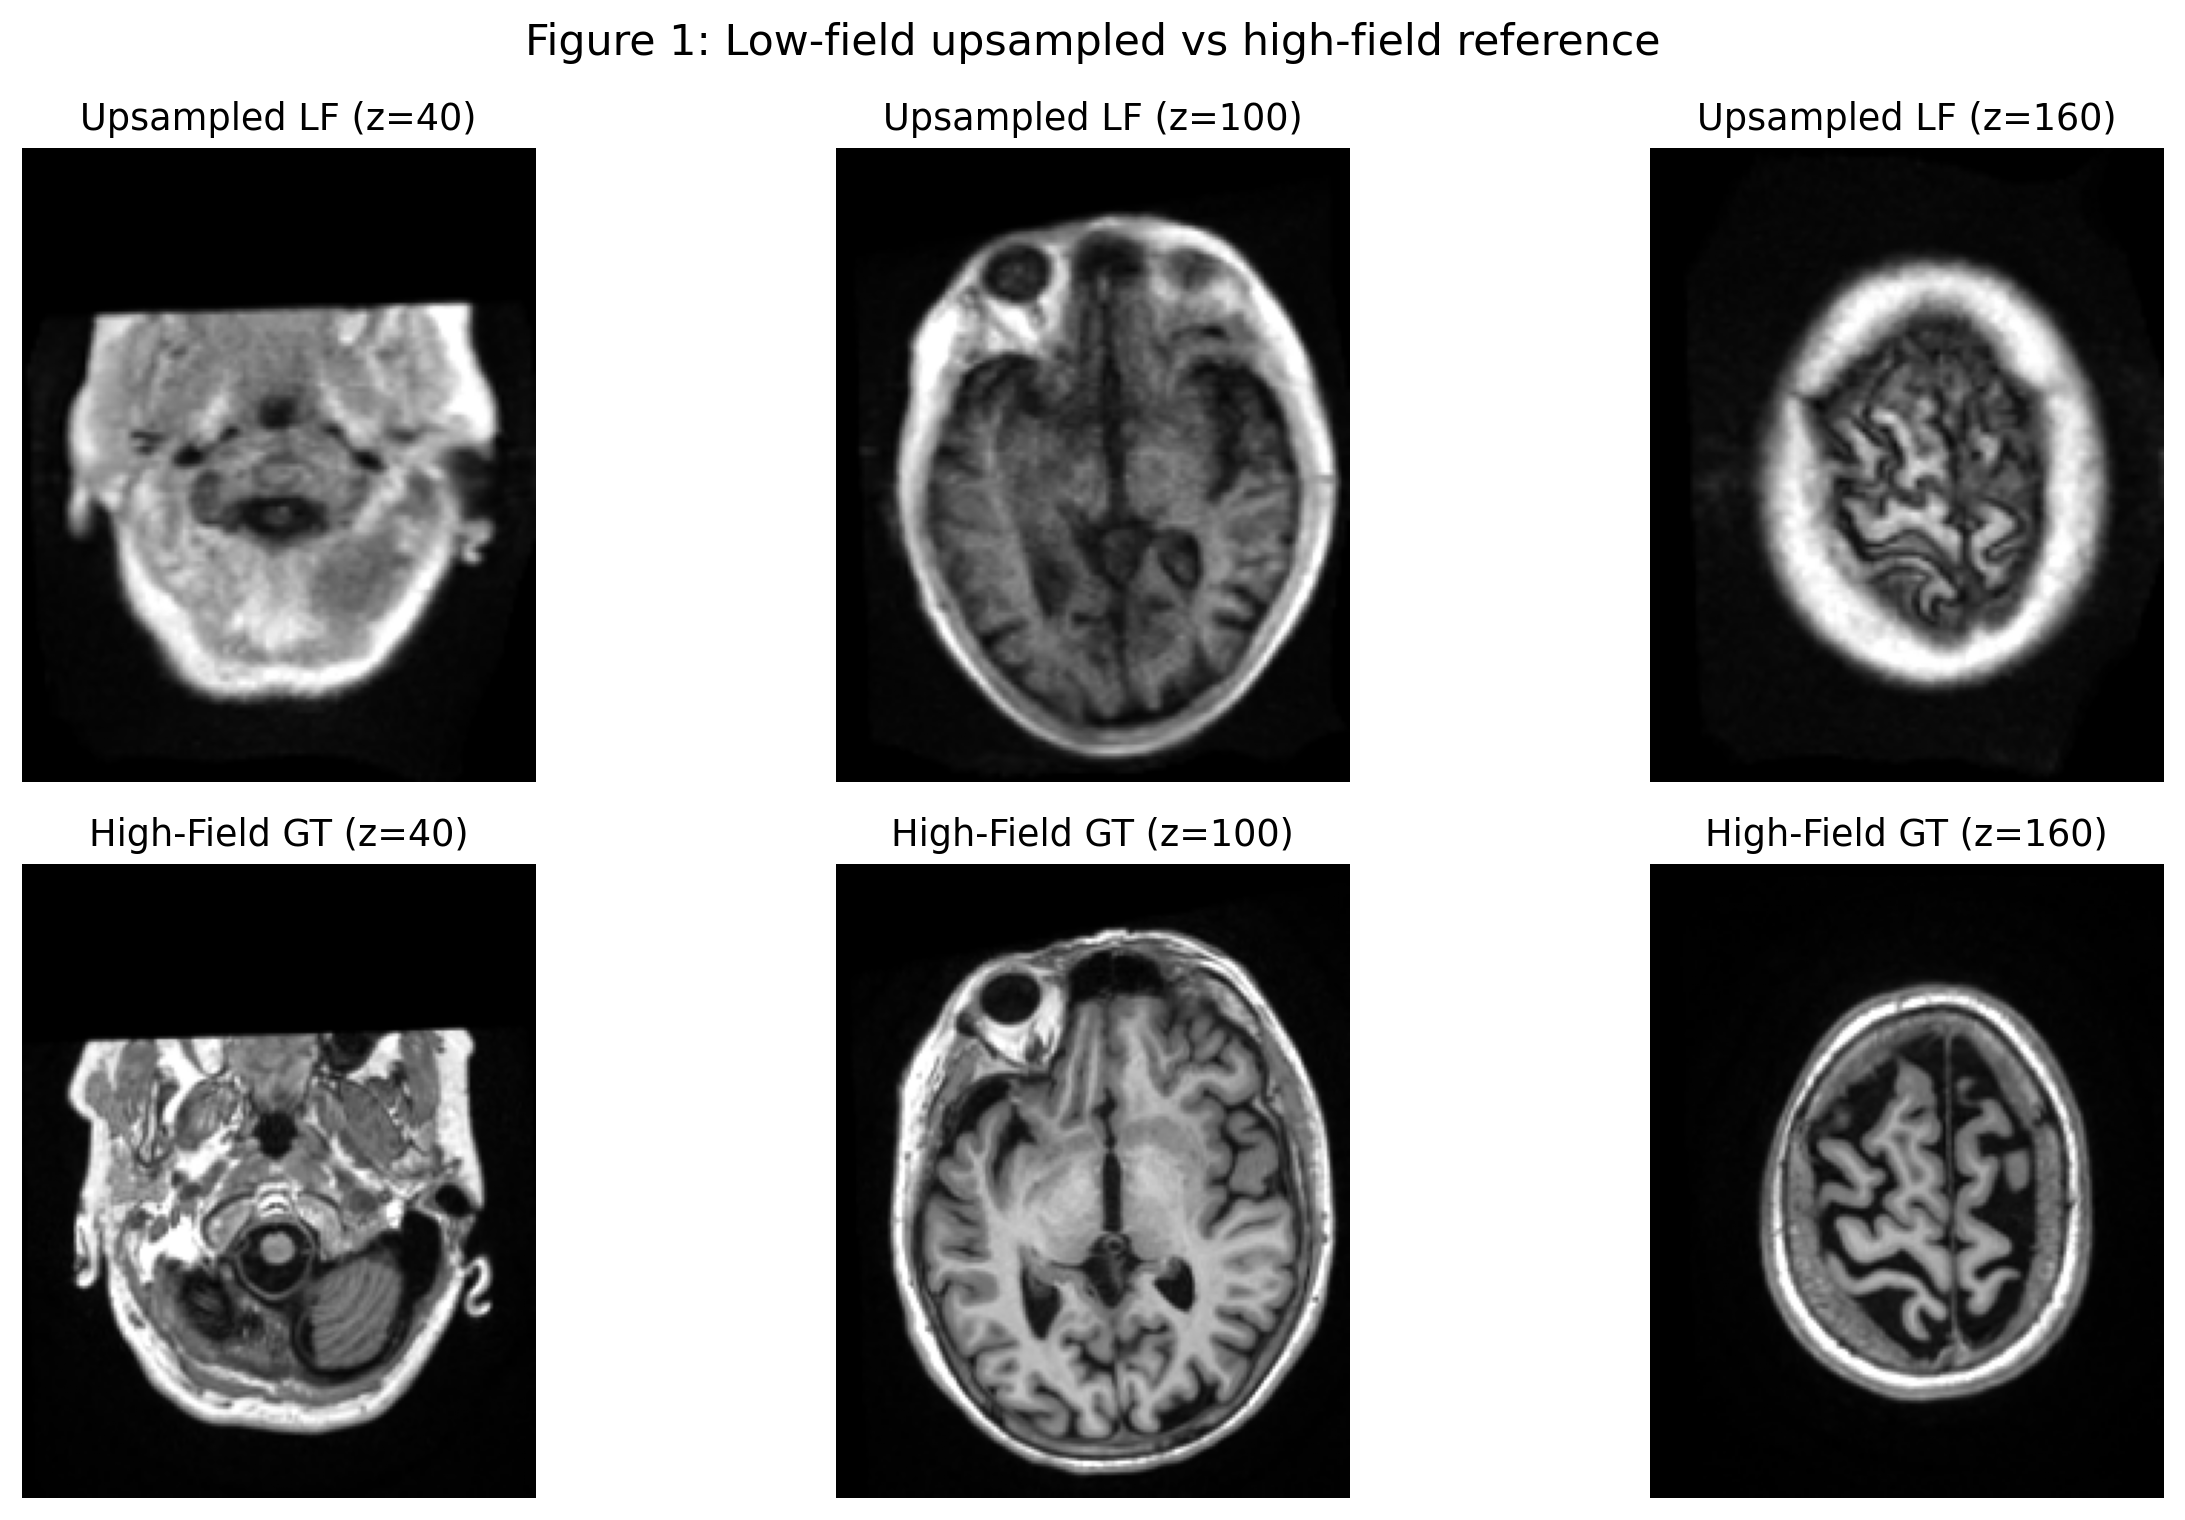
\includegraphics[width=0.95\linewidth]{figs/fig1.png}
    \caption{\textbf{Figure 1:} Side-by-side comparison of upsampled low-field and high-field axial slices at representative z-positions, illustrating the quality gap in SNR, sharpness, and contrast that the model must bridge. \textit{(Placeholder for image)}}
\end{figure}

\subsection{Augmentation}
During training, we applied random $160 \times 160$ crops (enabling $90^\circ$ rotations despite the non-square native slice dimensions of $179 \times 221$), random horizontal and vertical flips, random $90^\circ$ rotations, random intensity scaling in [0.9, 1.1] with probability 0.5, and additive Gaussian noise with standard deviation 0.01 at probability 0.3. At inference, full-resolution slices were used without cropping.

\subsection{Validation Strategy}
Finding a reliable validation strategy was a significant challenge given the extremely small dataset. We explored three approaches before settling on a final configuration. First, we attempted training on all 18 volumes with no holdout, relying solely on the Kaggle leaderboard for evaluation; this provided no signal during training and made it impossible to detect overfitting or guide early stopping. Second, we experimented with synthetic data expansion using the IXI dataset ($\sim$580 high-field T1 volumes): we applied degradation operations (downsampling, Rician noise, Gaussian blur, contrast adjustment) to simulate low-field inputs and used these synthetic pairs for pre-training followed by fine-tuning on the real 18 volumes. However, our synthetic degradation did not accurately reproduce the true characteristics of 64mT acquisitions, and models trained with synthetic data performed worse than those trained on real data alone. Ultimately, we held out samples 017 and 018 as a validation set (16 training / 2 validation volumes), which provided enough signal for early stopping and hyperparameter decisions.

\section{Methods}

\subsection{Problem Formulation}
The task is a paired image enhancement problem: given an input low-field volume $x \in \mathbb{R}^{112 \times 138 \times 40}$, produce an enhanced output $\hat{y} \in \mathbb{R}^{179 \times 221 \times 200}$ that closely matches the high-field target $y$. This requires both spatial super-resolution (a roughly $1.6\times$ increase in each spatial dimension and $5\times$ in the slice direction) and quality enhancement. Rather than operating on entire 3D volumes, we decompose this into a slice-wise prediction problem: for each axial slice index $z$, predict the high-field slice $y[:,:,z]$ from a stack of neighboring upsampled low-field slices.

\subsection{Failed Approach: 3D ESRGAN}
Our initial approach was a 3D Enhanced Super-Resolution Generative Adversarial Network, consisting of a 3D Residual-in-Residual Dense Block (RRDB) generator and a 3D relativistic PatchGAN discriminator with spectral normalization. Training followed a three-phase curriculum: L1+SSIM pre-training, GAN fine-tuning with adversarial and perceptual losses, and a final metric-focused tuning stage. The model was trained on $64^3$ patches with a batch size of 2.

This approach scored approximately 0.373 on the Phase 1 metric (0.5$\times$SSIM + 0.5$\times$PSNR/50), substantially below the bicubic baseline of 0.456. Two factors drove this failure. First, 3D convolutions across the full RRDB architecture produced far too many parameters for 18 training volumes, leading to severe overfitting. Second, adversarial training was unstable with so few samples --- the discriminator quickly memorized the training distribution and provided no useful gradient signal, while the generator outputs degraded in quality during the GAN phase.

\subsection{Primary Approach: 2.5D Residual U-Net}
Based on the lessons from the 3D ESRGAN, we adopted a 2.5D U-Net architecture \cite{ronneberger2015u} that processes 2D axial slices with z-axis context from neighboring slices. The input is a stack of 5 adjacent axial slices from the trilinear-upsampled low-field volume (shape: $5 \times 179 \times 221$), and the output is the predicted center high-field slice ($1 \times 179 \times 221$).

The encoder consists of four stages with channel progression $5 \rightarrow 64 \rightarrow 128 \rightarrow 256 \rightarrow 512$, with max-pooling between stages. A bottleneck block operates at 1024 channels. The decoder mirrors the encoder using bilinear upsampling (rather than transposed convolutions, to gracefully handle the non-power-of-2 spatial dimensions) followed by concatenation with skip connections from the corresponding encoder stage, producing channel progression $512 \rightarrow 256 \rightarrow 128 \rightarrow 64$. A final $1 \times 1$ convolution maps to a single output channel. The model has approximately 31.4M parameters with Kaiming normal initialization.

\begin{figure}[H]
    \centering
    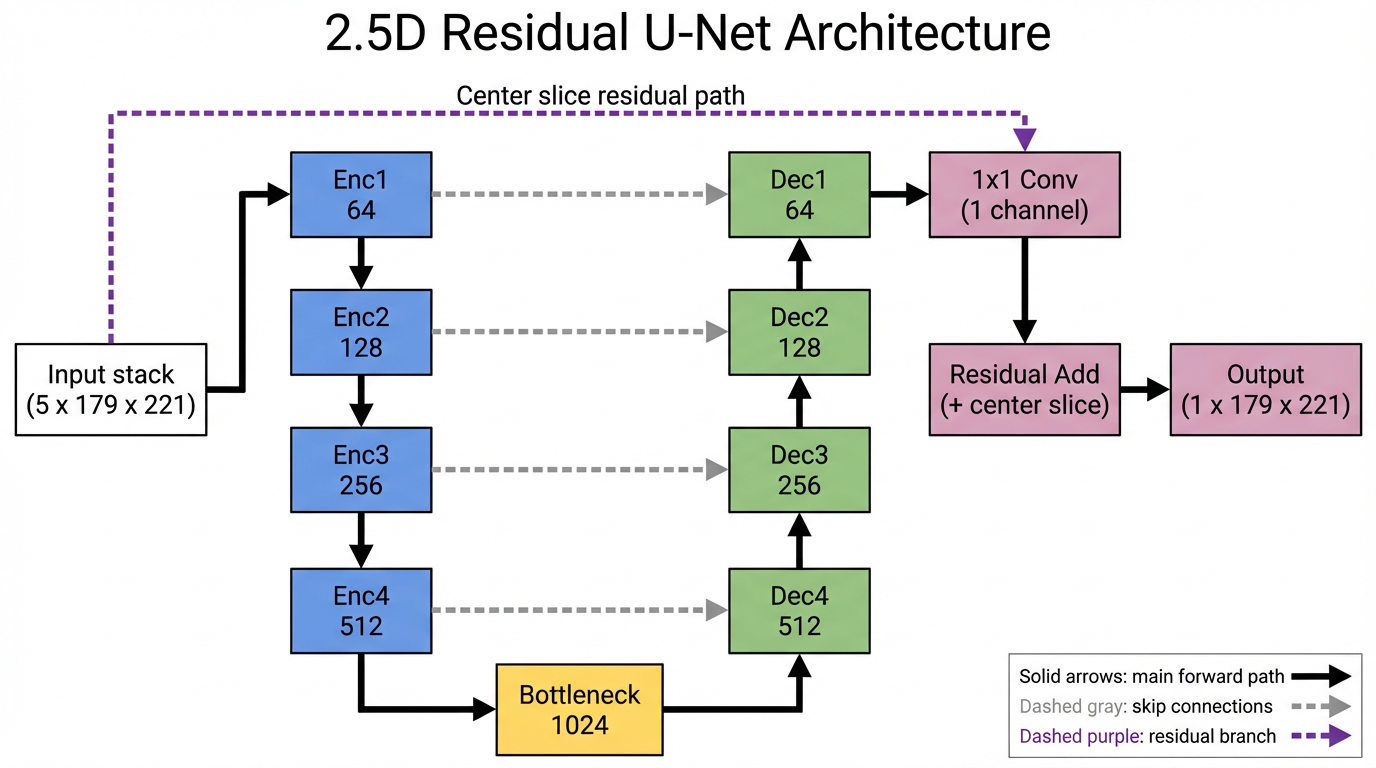
\includegraphics[width=0.95\linewidth]{figs/fig2.png}
    \caption{\textbf{Figure 2:} Architecture diagram of the 2.5D U-Net showing the encoder-decoder structure with skip connections and the residual connection from the center input slice. \textit{(Placeholder for image)}}
\end{figure}

A key design choice is residual learning: the network output is added to the center input slice, so the model learns only the enhancement residual (the difference between the upsampled low-field and high-field images) rather than reconstructing the full image from scratch. This stabilizes training because the input and target are already structurally similar after trilinear upsampling, and the residual is a smaller, easier-to-learn signal.

\subsection{Loss Functions}
We employed two loss functions jointly during training.

Charbonnier L1 loss provides a smooth approximation to L1 that avoids the non-differentiable point at zero:
$$\mathcal{L}_{\text{Char}}(\hat{y}, y) = \sqrt{(\hat{y} - y)^2 + \varepsilon^2}$$
where $\varepsilon$ is a small constant. This encourages pixel-accurate reconstruction while being less sensitive to outliers than L2 and producing smoother gradients near zero than standard L1.

Competition-matched SSIM loss directly optimizes the evaluation metric. For the Phase 1 metric, we implemented global SSIM (computed over entire image statistics rather than sliding windows) with constants $C_1 = 0.01^2$ and $C_2 = 0.03^2$, applied to slices independently normalized to [0, 1]. For Phase 2, we replaced this with MS-SSIM loss \cite{wang2003multiscale} using 5 scales with $11 \times 11$ Gaussian windows ($\sigma = 1.5$) and the standard perceptual weights. MS-SSIM captures structural similarity at multiple spatial resolutions --- lower resolutions emphasize global anatomy while higher resolutions focus on edges and textures.

The total loss for the Phase 2 U-Net was weighted as $0.16 \times L1 + 0.84 \times \text{MS-SSIM}$, reflecting the importance of the competition metric.

\subsection{Exploratory Approach: Conditional DDPM}
Regression models such as the U-Net minimize expected loss by averaging over the conditional distribution $p(\text{HF}|\text{LF})$, which regresses toward the conditional mean and tends to produce blurry outputs. MS-SSIM penalizes blur at fine scales more heavily than pixel-wise metrics, motivating exploration of generative models that can produce sharper samples.

We implemented a conditional DDPM following the SR3 framework \cite{saharia2022image}. The model concatenates the noisy high-field slice with 5 upsampled low-field conditioning slices as input (6 channels total), uses sinusoidal time embeddings with an MLP projection (dimension 256), and predicts the noise $\epsilon$ added at each diffusion timestep. The architecture is a U-Net with GroupNorm (not BatchNorm, which is incompatible with DDPM due to the mixture of noise levels within each batch) and SiLU activations, totaling $\sim$32.7M parameters. Training minimizes MSE between predicted and true noise, with an auxiliary image-space loss ($0.84 \times \text{MS-SSIM} + 0.16 \times L1$) weighted by SNR and applied to the predicted clean image $\hat{x}_0$. Inference uses DDIM sampling with 50 steps and $\eta = 0$ for deterministic generation.

In our configuration, the diffusion model did not outperform the U-Net. We attribute this to the substantial hyperparameter sensitivity of diffusion training (noise schedule, EMA decay rate, auxiliary loss weighting, number of sampling steps) combined with the limited time and compute budget available for tuning. 

\section{Results} 

\subsection{Training Details}
All training was performed on the NYU High Performance Computing cluster. Table 2 summarizes the hyperparameters for the best-performing 2.5D U-Net configuration. Each training run took approximately 2 hours.

\begin{table}[H]
\centering
\caption{Training hyperparameters for the best 2.5D U-Net.}
\begin{tabular}{ll}
\toprule
\textbf{Setting} & \textbf{Value} \\
\midrule
Optimizer & AdamW ($\beta_1=0.9$, $\beta_2=0.99$, weight decay=1e-4) \\
Learning rate & 1e-3 $\rightarrow$ 1e-6 (cosine annealing, 500-step linear warmup) \\
Batch size & 16 \\
Epochs & 400 \\
Loss weights & 0.16 $\times$ Charbonnier L1 + 0.84 $\times$ MS-SSIM \\
Mixed precision & Enabled (AMP) \\
EMA decay & 0.999 \\
Gradient clipping & max norm = 1.0 \\
Validation holdout & Samples 017, 018 \\
\bottomrule
\end{tabular}
\end{table}

\subsection{Results Summary}
Table 3 presents results across all approaches and both competition phases. The competition metric changed from a composite SSIM+PSNR score to pure MS-SSIM during the project.

\begin{table}[H]
\centering
\caption{Leaderboard results across approaches and competition phases. The 2.5D U-Net with MS-SSIM loss substantially outperformed the baseline and approached the SOTA reference.}
\begin{tabular}{lllll}
\toprule
\textbf{Model} & \textbf{Metric} & \textbf{Public} & \textbf{Private} & \textbf{Validation (internal)} \\
\midrule
Bicubic baseline & SSIM+PSNR & --- & 0.456 & --- \\
3D ESRGAN & SSIM+PSNR & --- & $\sim$0.373 & --- \\
2.5D U-Net (best) & SSIM+PSNR & 0.5214 & 0.5185 & --- \\
Bicubic baseline & MS-SSIM & 0.5130 & 0.5153 & --- \\
2.5D U-Net (best) & MS-SSIM & 0.6063 & 0.6126 & 0.6943 \\
SOTA reference (diffusion) & MS-SSIM & 0.6399 & 0.6343 & --- \\
\bottomrule
\end{tabular}
\end{table}

The 2.5D U-Net improved over the bicubic baseline by 18.2\% on the Phase 1 metric (private) and by 18.9\% on the Phase 2 MS-SSIM metric (private). Notably, ensemble methods (averaging predictions from multiple seeds) did not improve over the best single model during Phase 1, and test-time augmentation (horizontal/vertical flip averaging) did not yield gains in the final submission.

\subsection{Qualitative Results}

\begin{figure}[H]
    \centering
    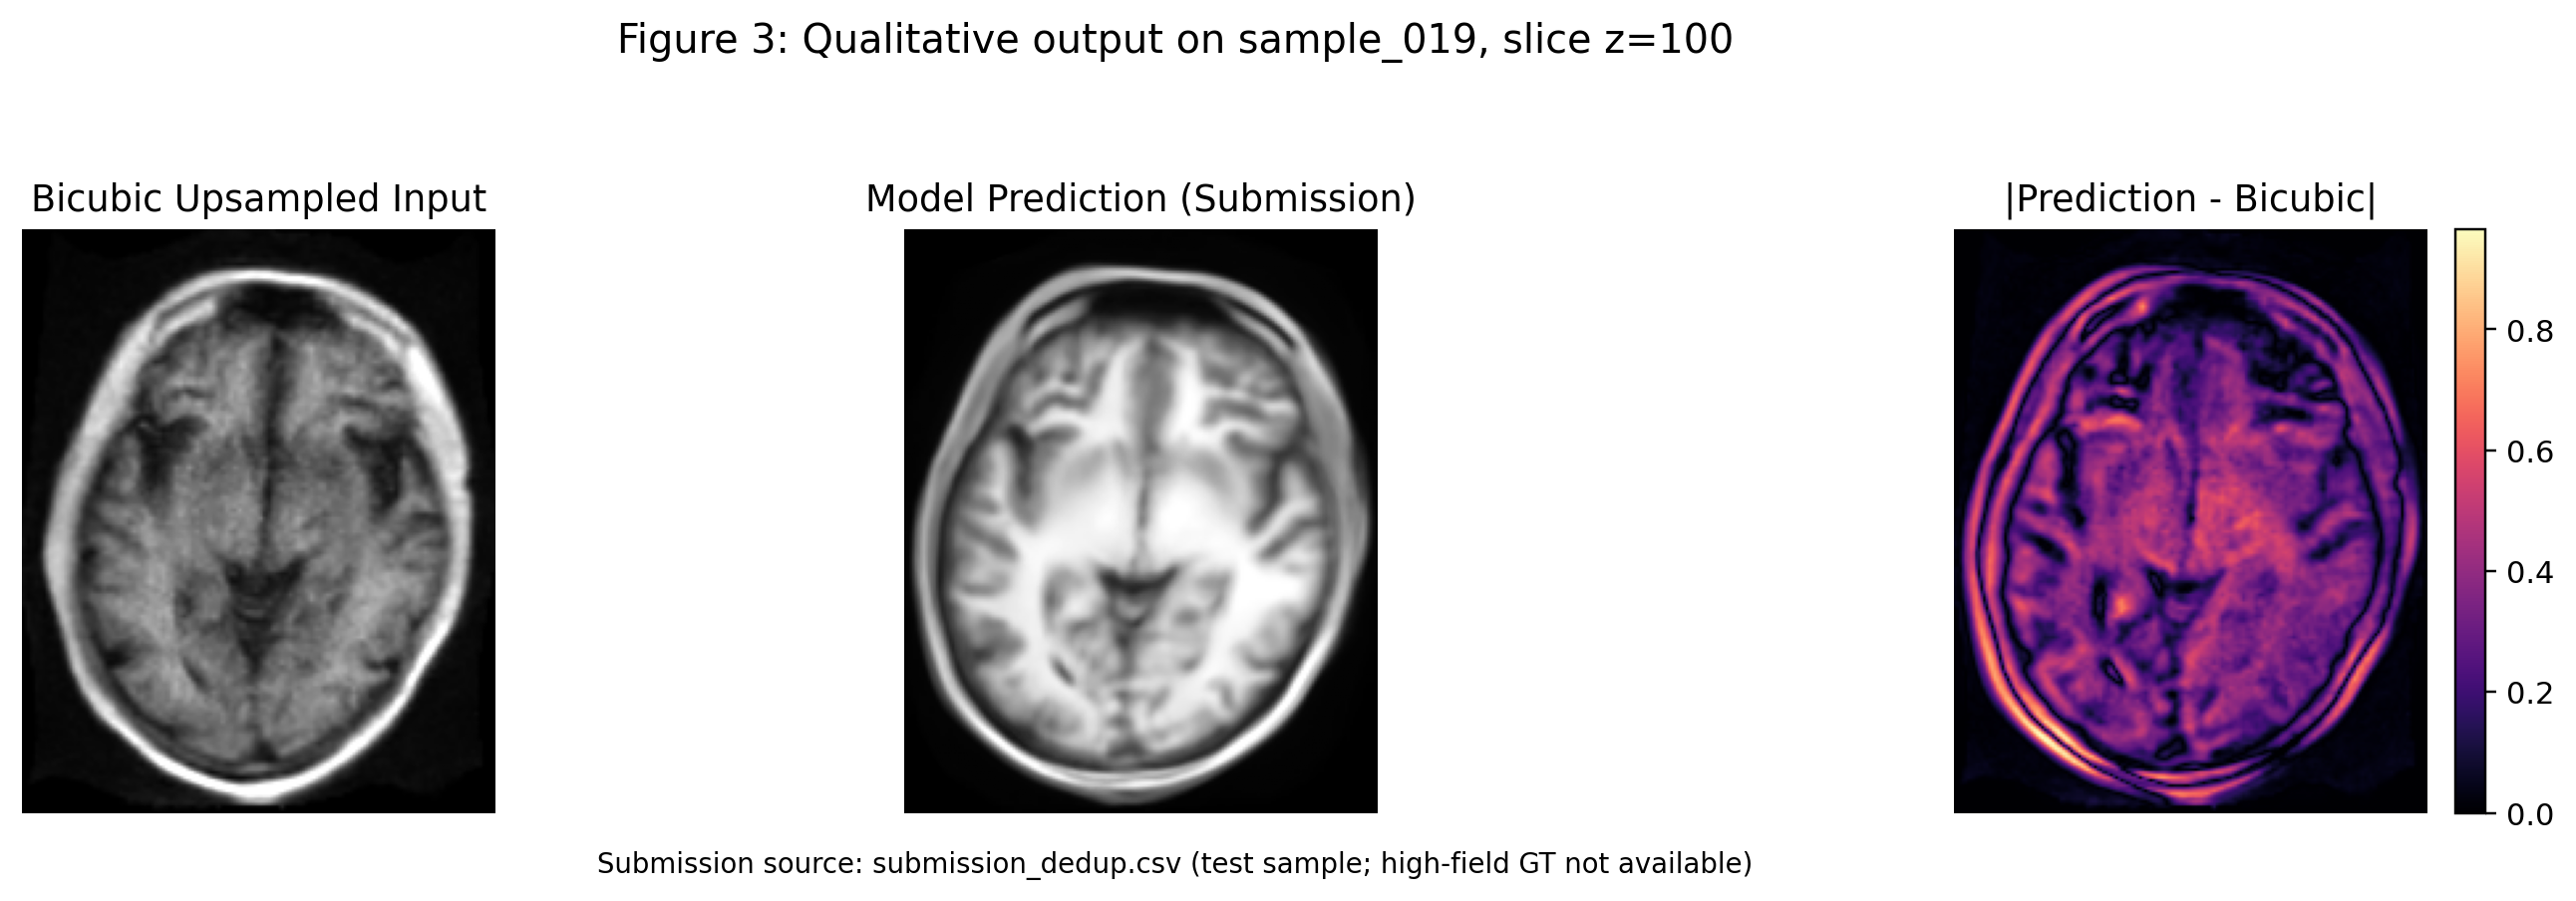
\includegraphics[width=0.95\linewidth]{figs/fig3.png}
    \caption{\textbf{Figure 3:} Visual comparison of a representative axial slice showing (left) bicubic upsampled low-field input, (center) 2.5D U-Net prediction, and (right) high-field ground truth. The U-Net output shows improved contrast, reduced noise, and sharper tissue boundaries compared to the bicubic baseline. \textit{(Placeholder for image)}}
\end{figure}

\begin{figure}[H]
    \centering
    \subfigure[U-Net Phase 2 v4 training metrics]{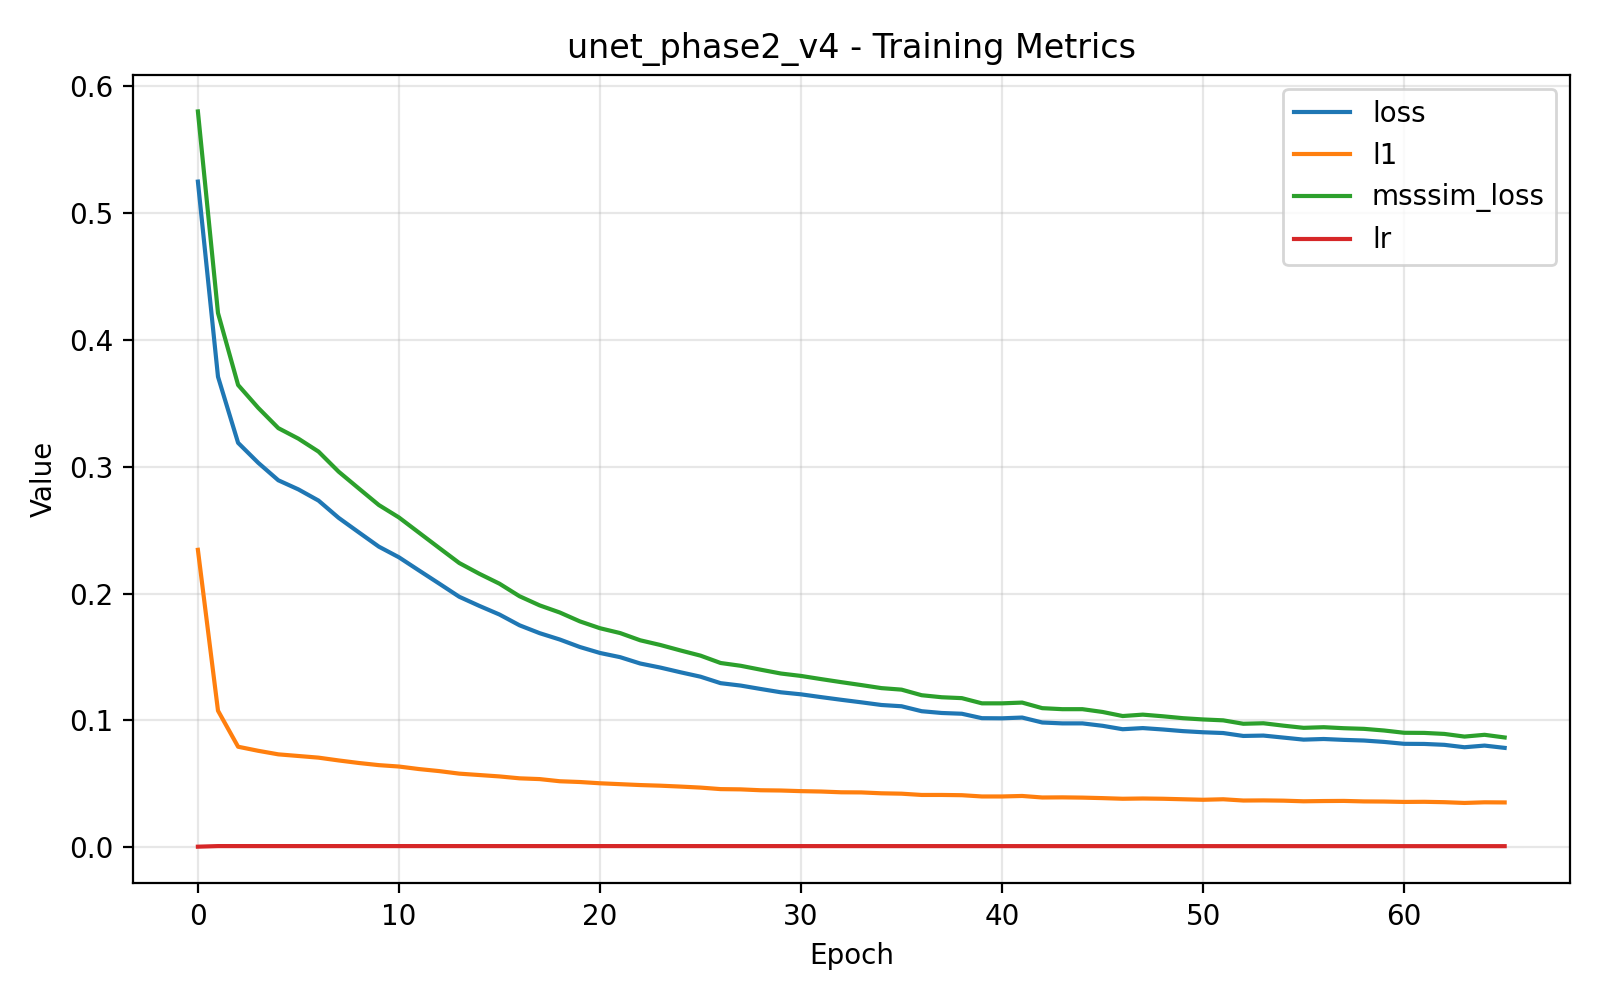
\includegraphics[width=0.48\linewidth]{log_plots/unet_phase2_v4_train_metrics.png}}
    \hfill
    \subfigure[U-Net Phase 2 v4 validation MS-SSIM]{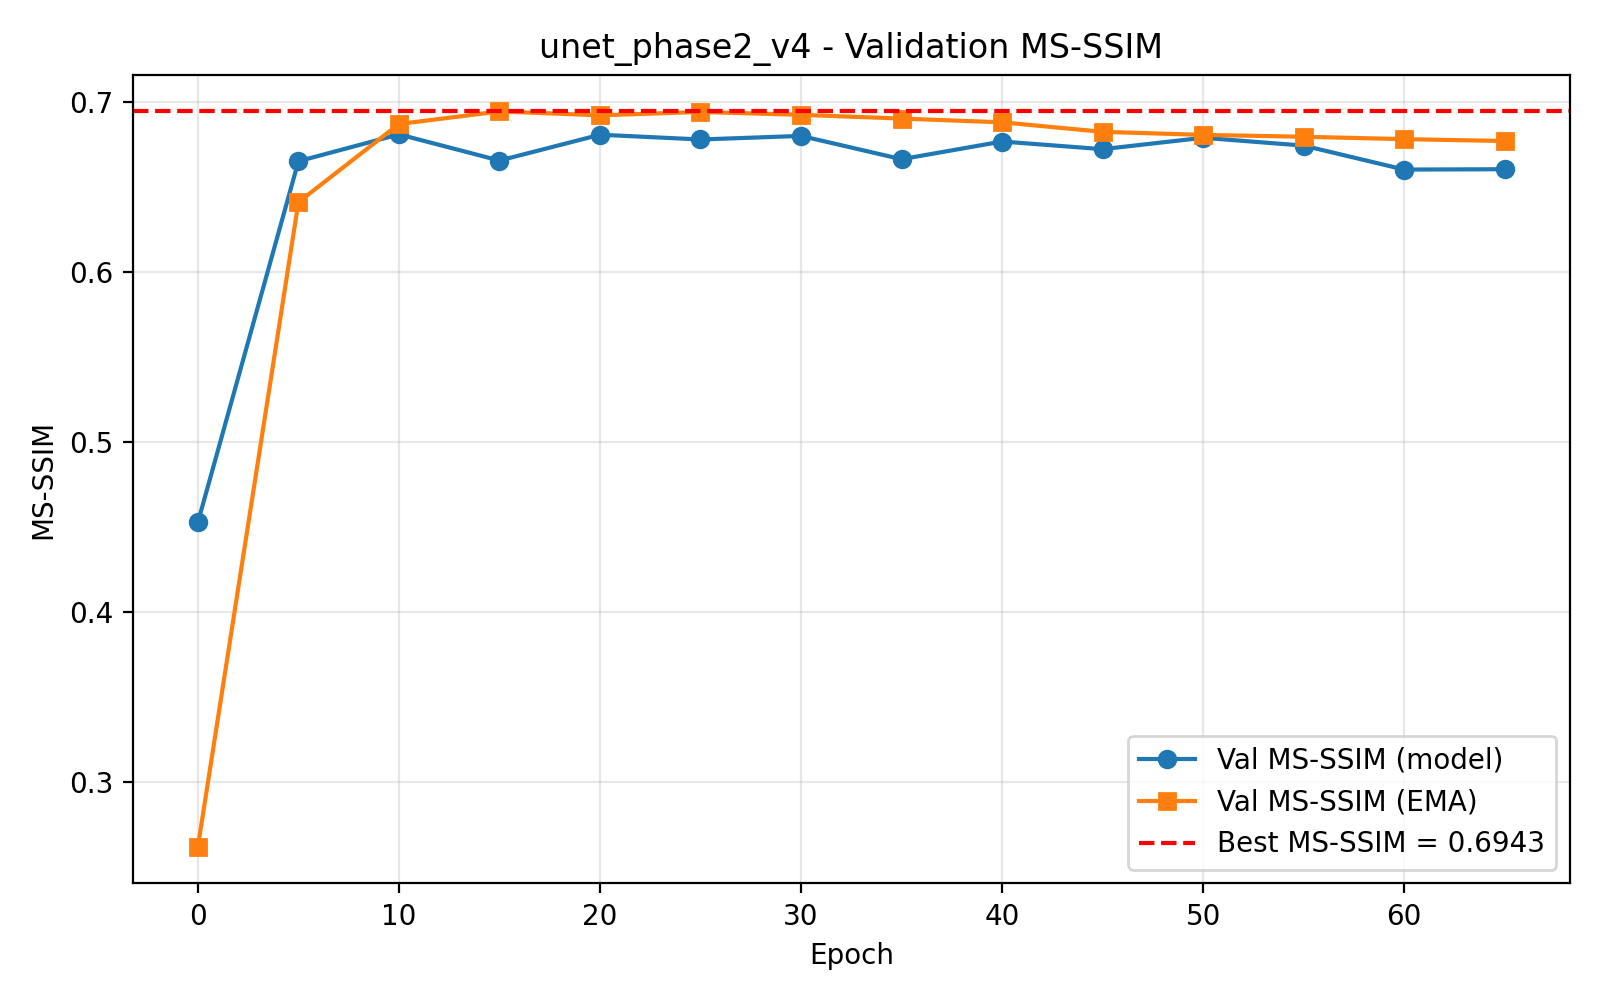
\includegraphics[width=0.48\linewidth]{log_plots/unet_phase2_v4_val_msssim.png}}
    \caption{\textbf{Figure 4:} Training dynamics for the best-performing 2.5D U-Net configuration.}
\end{figure}

\begin{figure}[H]
    \centering
    \subfigure[Diffusion base config training metrics]{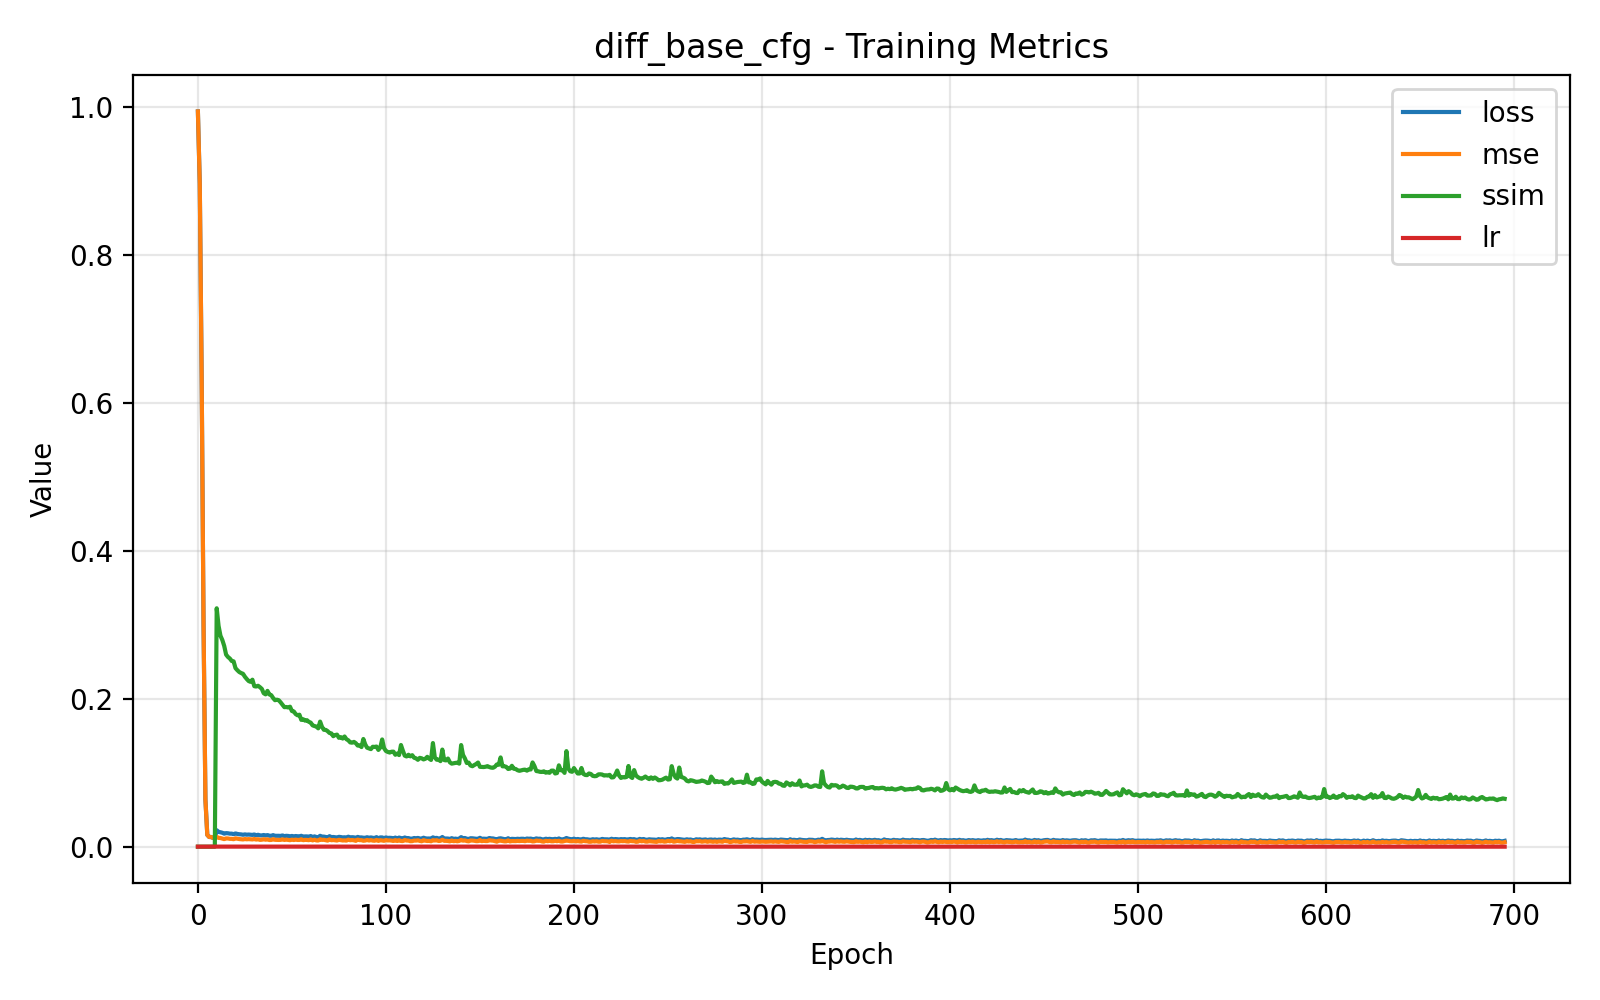
\includegraphics[width=0.48\linewidth]{log_plots/diff_base_cfg_train_metrics.png}}
    \hfill
    \subfigure[Diffusion base config validation MS-SSIM]{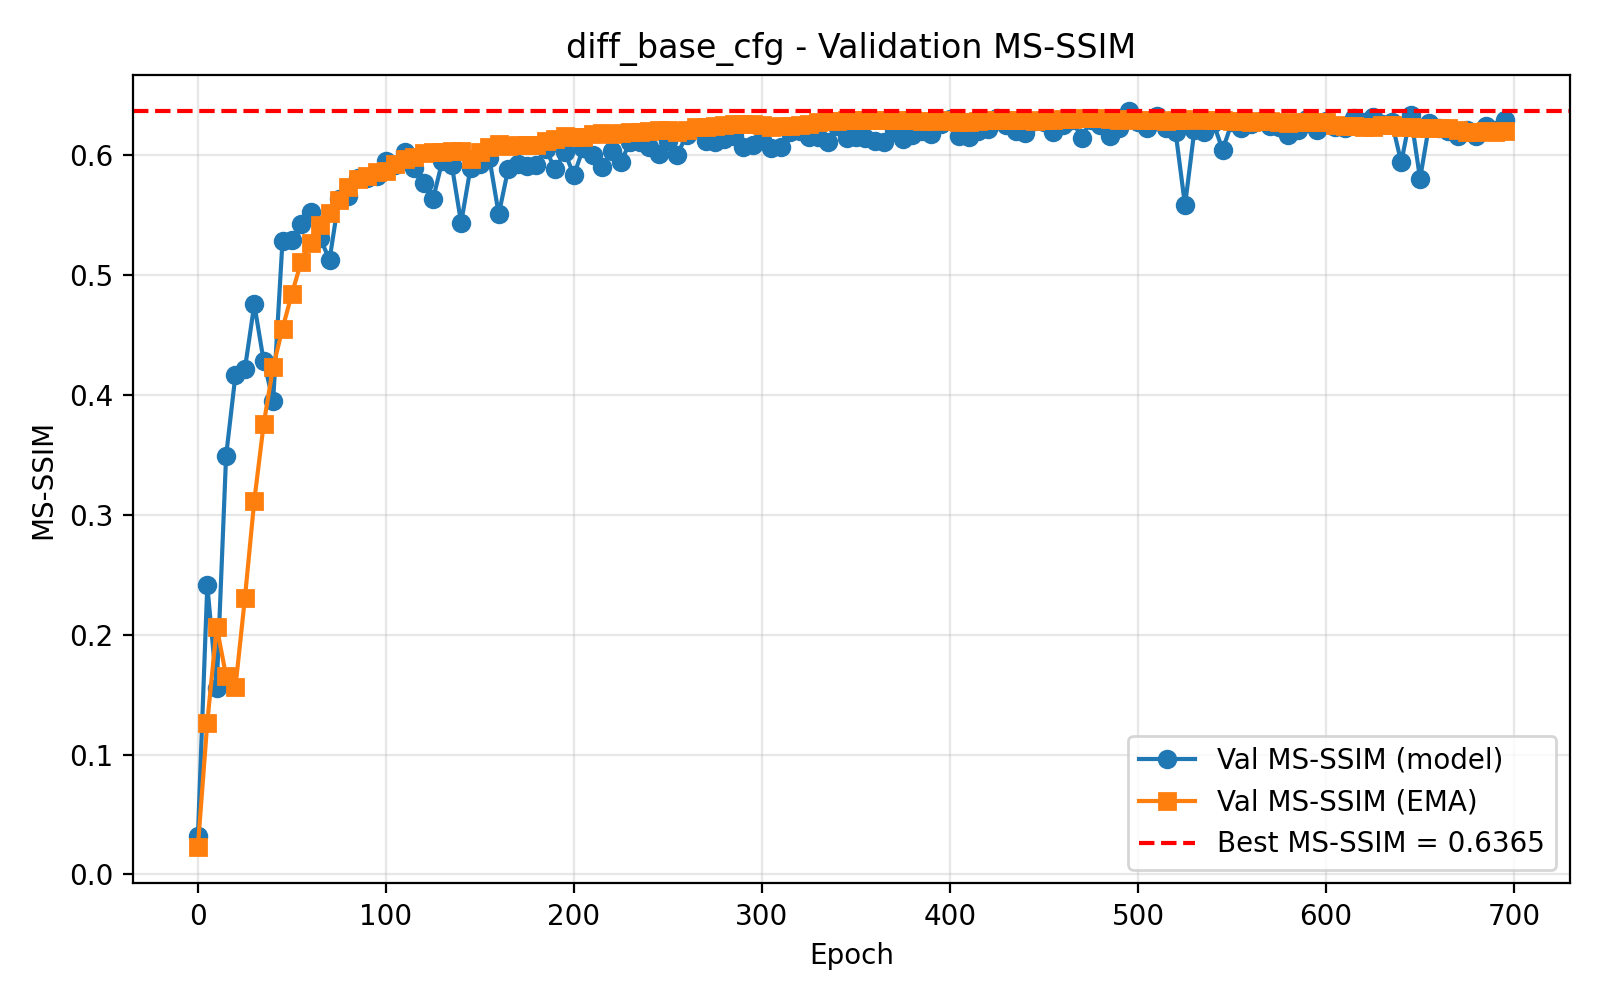
\includegraphics[width=0.48\linewidth]{log_plots/diff_base_cfg_val_msssim.png}}
    \caption{\textbf{Figure 5:} Training dynamics for the conditional diffusion baseline run.}
\end{figure}

\section{LLM Prompts}
Large language models were used to assist with code generation for the training pipeline, data loading utilities, and loss function implementations. In each case, the model was provided with detailed architectural specifications, dataset format descriptions, and target behavior before generating code. The LLM was not used for architectural design decisions or experimental strategy, which were guided by the course suggestions and iterative experimentation. A representative prompt and output are attached with the code submission.

\section{Conclusions}
This project explored multiple deep learning approaches for enhancing low-field (64mT) brain MRI to approximate high-field (3T) quality. Several key lessons emerged from the experimental process:

\begin{itemize}
    \item \textbf{Adversarial training is counterproductive with extremely limited data.} The 3D ESRGAN performed worse than simple bicubic interpolation when trained on only 18 volumes.
    \item \textbf{The 2.5D slice-based formulation provides the right balance of context and data efficiency.} By processing stacks of adjacent axial slices rather than full 3D volumes, the effective training set grows from 18 volumes to 3,600 slice examples.
    \item \textbf{Synthetic data expansion requires careful domain-specific calibration.} Models pre-trained on synthetic pairs performed worse than those trained on real data alone.
    \item \textbf{Diffusion models are theoretically well-motivated but demand careful implementation and extensive tuning.} Our SR3-style DDPM required debugging and tuning, and still did not surpass the simpler U-Net within the available time.
\end{itemize}

Looking forward, more thorough exploration of the DDPM framework with a wider hyperparameter sweep could potentially close the gap to the SOTA reference score. Better synthetic degradation modeling could also unlock the value of large external datasets.

\section{Author Contributions}
This project was completed individually by Chetan [Last Name].

\section{References}

\begin{thebibliography}{99}

\bibitem{saharia2022image} 
Saharia, C., Ho, J., Chan, W., et al. (2022). 
\textit{Image Super-Resolution via Iterative Refinement}. IEEE TPAMI.

\bibitem{wang2018esrgan} 
Wang, X., Yu, K., Wu, S., et al. (2018). 
\textit{ESRGAN: Enhanced Super-Resolution Generative Adversarial Networks}. ECCV Workshops.

\bibitem{wang2003multiscale} 
Wang, Z., Simoncelli, E.P., Bovik, A.C. (2003). 
\textit{Multiscale Structural Similarity for Image Quality Assessment}. Asilomar Conference on Signals, Systems \& Computers.

\bibitem{ronneberger2015u} 
Ronneberger, O., Fischer, P., Brox, T. (2015). 
\textit{U-Net: Convolutional Networks for Biomedical Image Segmentation}. MICCAI.

\end{thebibliography}

% \printbibliography
%%%%%%%%%%%%%%%%%%%%%%%%%%%%%%%%%%%%%%%%%%%%%%%%%%%%%%%%%%%%

\end{document}